\documentclass[12pt]{article}
\usepackage{geometry}                % See geometry.pdf to learn the layout options. There are lots.
\geometry{letterpaper}                   % ... or a4paper or a5paper or ... 
%\geometry{landscape}                % Activate for for rotated page geometry
\usepackage[parfill]{parskip}    % Activate to begin paragraphs with an empty line rather than an indent
\usepackage{graphicx}
\usepackage{amsmath,amssymb}
\usepackage{enumitem, multicol, tasks}
\usepackage{fourier}
\usepackage{pgfplots}
\pagestyle{empty}

\usepackage{epstopdf}
\DeclareGraphicsRule{.tif}{png}{.png}{`convert #1 `dirname #1`/`basename #1 .tif`.png}

\topmargin=-1in
\textheight=10in
\begin{document}
Math 109 S26  \hfill Name: \enspace\rule{2in}{0.4pt}\\
Quiz 3A

\begin{enumerate}[leftmargin=*]
\item The derivative $f'(a)$ of a function $f$ at the point $x=a$ is defined as
\[
f'(a) = \lim_{h\to 0}\frac{f(a+h)-f(a)}{h}.
\]
Let $f(x)=x^2+2x$. Find $f'(1)$ and use it to find the equation of the tangent line to the graph of $y=f(x)$ at $x=1$.

\vspace{3.5in}
\item Here is the graph of a function $g(x)$. Determine the values of $x$ where $g'(x)$ is positive, negative, and zero (make sure you do this first!), and use it to sketch a graph of $g'(x)$.

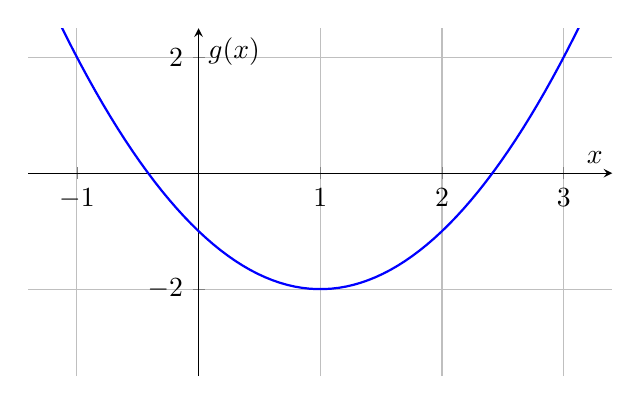
\begin{tikzpicture}
  \begin{axis}[
    axis lines=middle,
    xlabel={$x$},
    ylabel={$g(x)$},
    xmin=-1, xmax=3,
    ymin=-3, ymax=2,
    domain=-2:4,
    samples=100,
    grid=both,
    enlargelimits=true,
    width=9cm,
    height=6cm
  ]
    % Plot the parabola
    \addplot[blue, thick] {(x-1)^2 -2};
   \end{axis}
 \end{tikzpicture}

\end{enumerate}
%%%%%%%%%%%%%%%%
\newpage
%%%%%%%%%%%%%%%%

Math 109 S26  \hfill Name: \enspace\rule{2in}{0.4pt}\\
Quiz 3B

\begin{enumerate}[leftmargin=*]
\item
The derivative $f'(a)$ of a function $f$ at the point $x=a$ is defined as
\[
f'(a) = \lim_{h\to 0}\frac{f(a+h)-f(a)}{h}.
\]
Let $f(x)=x^2-3x$. Find $f'(1)$ and use it to find the equation of the tangent line to the graph of $y=f(x)$ at $x=1$.

\vspace{3.5in}
\item Here is the graph of a function $g(x)$. Determine the values of $x$ where $g'(x)$ is positive, negative, and zero (make sure you do this first!), and use it to sketch a graph of $g'(x)$.

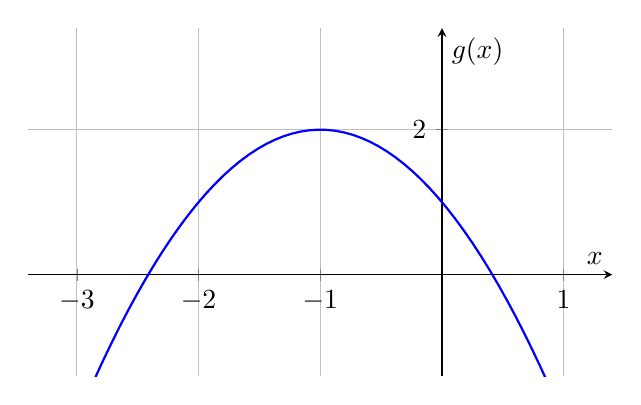
\begin{tikzpicture}
  \begin{axis}[
    axis lines=middle,
    xlabel={$x$},
    ylabel={$g(x)$},
    xmin=-3, xmax=1,
    ymin=-1, ymax=3,
    domain=-3:4,
    samples=100,
    grid=both,
    enlargelimits=true,
    width=9cm,
    height=6cm
  ]
    % Plot the parabola
    \addplot[blue, thick] {-(x+1)^2 +2};
   \end{axis}
 \end{tikzpicture}

\end{enumerate}
%%%%%%%%%%%%
\end{document}
%%%%%%%%%%%%%

